\chapter{Future work}\label{chapter:future-work}

This master thesis was primarily focused on implementing a prototypical micro-frontend architecture to replace AGnet's internal management software sometime in the future. The process examined whether using GraphQL with Apollo Client can bring performance improvements inside a micro-frontend architecture. The improvements with GraphQL should be implemented with two methods. First, a caching layer should be shared across all micro-frontends. Second, the GraphQL layer should remove fields from queries that are already stored inside the cache. Using a single cache instance for all micro-frontends leads to significant improvements regarding request size and response size. The second method of improving performance by reducing the fields of a query was auspicious, but in the prototype scenario, it did not bring significant improvements. The screen design and structure of the prototype follow the approach of a list view showing a table with some fields of every type. Moreover, a detail for every table row view mainly loads all fields of the type; however, the table view does not prefetch and store enough fields in the cache to make a difference in request and response size. Nevertheless, other applications with a different design might benefit from reducing queries with existing data. The following section explains a theoretical example of an application that might benefit from query reduction.

\subsubsection{Example of an e-commerce platform benefiting from query reduction and a shared cache layer}

This section describes a fictional application that could improve significantly using query reduction and a shared caching layer. The described application is an e-commerce platform, which has the same features as the prototypical micro-frontend architecture. The e-commerce application has multiple micro-frontends, each responsible for a different part of the shopping experience. The micro-frontends for an e-commerce application could include multiple widgets on the landing page, product browsing, product detail, shopping cart, checkout process, and order tracking. A possible journey through an e-commerce application is shown in Figure \ref{fig:future-work:flow-chart}.

\ifshowImages
\begin{figure}[H]
  \centering
  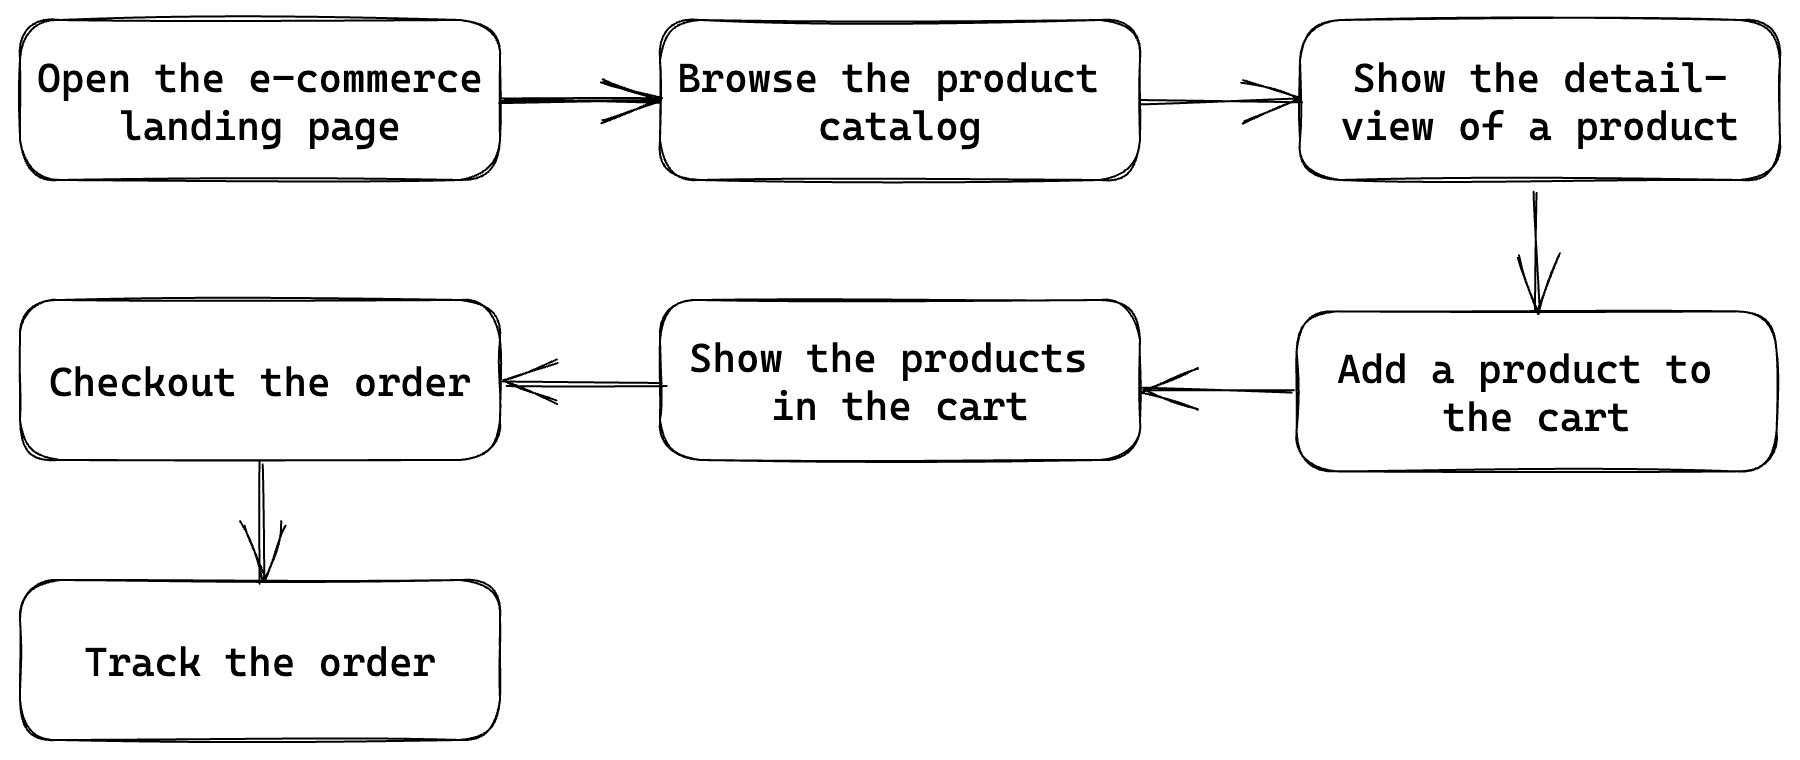
\includegraphics[width=0.8\linewidth]{images/future-work/flow-chart-e-commerce.png}
  \caption{A possible user journey through an e-commerce application.}\label{fig:future-work:flow-chart}
\end{figure}
\fi

\noindent The user starts by opening the landing page of the e-commerce platform. There the user sees a list of recommended products and a list of product categories. The images and some information about the most suggested products are loaded and stored inside the cache. The user clicks on a recommended category and is redirected to the product browsing page. The product browsing page shows a list of products in the selected category. The first products shown in the category are the same as on the landing page. Therefore, some data, including the product name, user rating, price, and image, can be reused from the cache. If the user scrolls down, the missing products are loaded from the server, rendered to the screen, and stored in the cache. Once the user finds a product they like, they can view the detail view. The detail view shows the product name, images, price, description, user rating, and reviews of other users. Much of the more significant data, like the product images which are shown on the page, can be reused from the cache and can therefore be used to render the page faster. Once the user finds a product they like, they can add it to their shopping cart. When the user is ready to purchase the items in their cart, they proceed to the checkout process. The checkout process shows the user's address, the selected products, and the price. The information on the products can be completely reused from the cache. The information about the user's address can be reused from the cache. They enter their shipping and billing information, choose a payment method, and review their order details. After submitting the order, the user sees a confirmation page with the order number, the ordered products, and the estimated delivery date. The user can track their order status and delivery progress. This information can also be fully reused from the cache if it is the same session.

\bigskip

\noindent This kind of application dramatically benefits from the shared caching layer and the mechanism of removing fields from a query already in the cache. Products are the most important citizen of the e-commerce application. The shared caching layer is just as important as in the micro-frontend prototype and enables the reuse of most information. The user sees the same products on the landing page, the product browsing page, the product detail page, the shopping cart, the checkout process, and the order summary. Therefore, the product data is stored in the cache and can be used and extended on every page, which also benefits the following pages.

\subsubsection{Further prototype development}

The current focus is the further development of micro-frontend architecture. The prototypical implementation, done in this master thesis, has implemented only a small subset of the functional requirements of the overall system. However, the basic setup that all micro-frontends must follow is defined and easily accessible. Creating, integrating, and configuring a new micro-frontend are also well-defined and follow a standardized principle. The process of creating, configuring and adding a new micro-frontend might be automated in the future with the help of Angular's Schematics\footnote{\url{https://angular.io/guide/schematics}}.
